%= <span class="free"></span>

\noindent One of the most important tasks for any aspiring developer---or any technical person generally---is setting up their computer as a \emph{development environment}, making it suitable for developing websites, web applications, and other software. \ledev\ is designed to complement the \href{http://www.learnenough.com/tutorials}{main Learn Enough sequence} and the \rort\ by putting all of the relevant material in one place.

This tutorial covers several options for setting up a dev environment, aimed at readers of varying levels of experience and sophistication. If you end up using one of the options shown in Section~\ref{sec:cloud_ide} or Section~\ref{sec:virtual_machine}, there is no minimum prerequisite for this tutorial other than general computer knowledge. If you want to follow the more challenging setup in Section~\ref{sec:native_os_setup}---which we recommend most readers tackle at some point---you should have a basic familiarity with the Unix command line (as covered in \lecl), and a familiarity with text editors and system configuration (as covered in \lete) is recommended.

Ebook versions of this tutorial are available for \href{https://www.softcover.io/email-capture/28fdb94f/learn_enough_dev_environment}{free at learnenough.com} and for \href{https://www.amazon.com/Learn-Enough-Dev-Environment-Dangerous-ebook/dp/B01MTEQJ6E}{99¢ at Amazon.com}.

\section{Dev environment options} % (fold)
\label{sec:dev_environment_options}

Our focus in this tutorial is on installing or otherwise enabling the following four fundamental tools of software development (Figure~\ref{fig:dev_environment}):
\begin{enumerate}
  \item Command line terminal (``shell'')
  \item Text editor
  \item Version control (Git)
  \item Programming languages (Ruby, etc.)
\end{enumerate}
For more information on these different types of software application, see \lecl, \lete, \leg, and \ler.

\begin{figure}
\begin{center}
\image{images/figures/dev_environment.png}
\end{center}
\caption{Typical elements of a dev environment.\label{fig:dev_environment}}
\end{figure}

When setting up a development environment, there are three different possibilities we recommend, listed in increasing order of difficulty:

\begin{enumerate}
  \item Cloud \href{https://en.wikipedia.org/wiki/Integrated_development_environment}{IDE}
  \item Virtual Machine (VM)
  \item Native OS (macOS, Linux, Windows)
\end{enumerate}

If you're relatively inexperienced, we recommend starting with the cloud IDE (Section~\ref{sec:cloud_ide}), as it has the least difficult setup process. The VM option is also relatively straightforward in principle (Section~\ref{sec:virtual_machine}), although the relevant files are large and can lead to confusing errors when trying to install, and some users may find that the user interface (UI) isn't as polished as the one on their native system.

\subsubsection{Native system} % (fold)
\label{sec:native_system}

While the IDE and VM options are great when you're just getting started, eventually it's important to be able to develop software on your native operating system (OS)\@. Unfortunately, setting up a fully functional native development environment can be a challenging and frustrating process\footnote{This is why it's such a bad idea to include a native dev setup at the beginning of a book like the \rortb. It's better to get started with the core material first, and tackle the native dev environment setup later. The switch over to a cloud IDE in the third edition of the \rortb\ was motivated by this realization.}---likely leaving ample opportunity to exercise your technical sophistication (Box~\ref{aside:technical_sophistication})---but it is an essential rite of passage for every aspiring technical wizard.

In order to tackle this difficult challenge, in Section~\ref{sec:native_os_setup} we'll discuss native OS setup for macOS, Linux, and Windows.

\begin{aside}
\label{aside:technical_sophistication}
\heading{Technical sophistication.}

\emph{Technical sophistication} is the ability to independently solve technical problems. In the context of installing a development environment, this means knowing to google the error message if something goes wrong, to try quitting and restarting an application (such as the command-line shell) to see if that fixes things, etc.

So many things can go wrong when setting up a development environment that there's rarely a general solution to the problem---you just have to keep applying your technical sophistication until you get everything to work. And if you do get stuck, don't worry too much about it---at some point or another, it happens to us all.

\end{aside}

% subsubsection native_system (end)

% section dev_environment_options (end)

\section{Cloud IDE}
\label{sec:cloud_ide}

The easiest dev environment option is a \emph{cloud IDE}, which is an integrated development environment in the \href{https://en.wikipedia.org/wiki/Cloud_computing}{cloud} that you access using the web browser of your choice. Although easy to activate, the resulting system is an industrial-grade development machine, not a toy. In addition, the cloud IDE automatically works cross-platform, since all you need is an ordinary web browser to use it (which every major OS provides).

There are several commercial options for running a cloud IDE, and as part of developing the \rort\ we partnered with \href{http://c9.io/}{Cloud9} (part of Amazon Web Services). The resulting environment is appropriate for Ruby on Rails web development, and as a matter of course includes all the elements mentioned in Section~\ref{sec:dev_environment_options}. In particular, AWS Cloud9 comes equipped with a command-line terminal and a text editor (including a filesystem navigator), as shown in Figure~\ref{fig:ide_anatomy}. Because each Cloud9 workspace provides a full working Linux system, it also automatically includes the Git version control system, as well as Ruby and several other programming languages.

\begin{figure}
\begin{center}
\image{images/figures/ide_anatomy_aws.png}
\end{center}
\caption{The anatomy of the cloud IDE.\label{fig:ide_anatomy}}
\end{figure}

Here are the steps for getting started with the cloud development environment:\footnote{Due to the constantly evolving nature of sites like AWS, details may vary; use your technical sophistication (Box~\ref{aside:technical_sophistication}) to resolve any discrepancies.}
\begin{enumerate}
\item Because Cloud9 is part of Amazon Web Services (AWS), if you already have an AWS account you can just \href{https://aws.amazon.com/}{sign in}.\footnote{https://aws.amazon.com/} To create a new Cloud9 workspace environment, go to the \href{https://console.aws.amazon.com/}{AWS console} and type ``Cloud9'' in the search box.
\item If you don't already have an AWS account, you should \href{https://www.railstutorial.org/cloud9-signup}{sign up for a free account at AWS Cloud9}.\footnote{https://www.railstutorial.org/cloud9-signup} In order to prevent abuse, AWS requires a valid credit card for signup, but the workspace is 100\% free (for a year as of this writing), and your card will not be charged. You might have to wait up to 24 hours for the account to be activated, but in my case it was ready in about ten minutes.
\item Once you've successfully gotten to the Cloud9 administrative page (Figure~\ref{fig:cloud9_page_aws}), keep clicking on ``Create environment'' until you find yourself on a page that looks like Figure~\ref{fig:cloud9_new_workspace}. Enter the information as shown there, then keep clicking the confirmation buttons until Cloud9 starts provisioning the IDE (Figure~\ref{fig:cloud9_ide_aws}). You may run into a warning message about being a ``root'' user, which you can safely ignore at this early stage. (If you're feeling up to it, you can implement the preferred method, called an Identity and Access Management (IAM) user, at this point. See \href{https://www.railstutorial.org/book/user_microposts#sec-image_upload_in_production}{Chapter 13 in the \href{https://www.railstutorial.org/}{\emph{Ruby on Rails Tutorial}}} for more information.)
\end{enumerate}

\begin{figure}
\begin{center}
\image{images/figures/cloud9_page_aws.png}
\end{center}
\caption{The administrative page for Cloud9.\label{fig:cloud9_page_aws}}
\end{figure}

\begin{figure}
\begin{center}
\image{images/figures/cloud9_name_environment.png}
\end{center}
\caption{Creating a new work environment at AWS Cloud9.\label{fig:cloud9_new_workspace}}
\end{figure}

\begin{figure}
\begin{center}
\image{images/figures/cloud9_ide_aws.png}
\end{center}
\caption{The default cloud IDE. \label{fig:cloud9_ide_aws}}
\end{figure}

Because using two spaces for indentation is a near-universal convention in Ruby, I also recommend changing the editor to use two spaces instead of the default four. As shown in Figure~\ref{fig:cloud9_two_spaces}, you can do this by clicking the gear icon in the upper right and then changing the ``Soft Tabs'' setting to~2. (Note that this takes effect immediately; you don't need to click a ``Save'' button.)


\begin{figure}
\begin{center}
\image{images/figures/cloud9_two_spaces_aws.png}
\end{center}
\caption{Setting Cloud9 to use two spaces for indentation.\label{fig:cloud9_two_spaces}}
\end{figure}

At this point, you're done! Although Internet access is required to use Cloud9, there is no alternative that combines so much power with such an easy setup.


\section{Virtual machine} % (fold)
\label{sec:virtual_machine}

A second option for setting up a development environment is a \emph{virtual machine}, or \emph{VM}, which is a fully functional computer system that runs inside the host system. In the case of the Learn Enough VM that we recommend, you can run a full Linux system right inside of macOS or Windows (or even Linux! \href{https://en.wikipedia.org/wiki/Turtles_all_the_way_down}{It's turtles all the way down} (Figure~\ref{fig:turtles}).\footnote{Image retrieved from https://upload.wikimedia.org/wikipedia/commons/4/47/River\_terrapin.jpg on 2017-01-24. Image is in the public domain.}).

\begin{figure}
\begin{center}
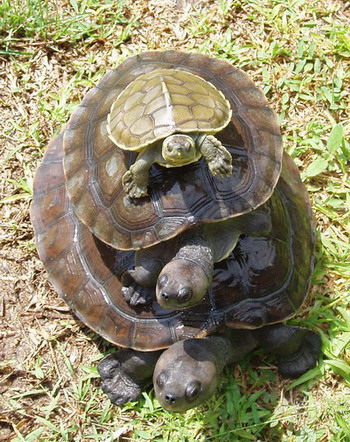
\includegraphics[width=5.5in]{images/figures/turtles.jpg}
\end{center}
\caption{It's turtles all the way down.\label{fig:turtles}}
\end{figure}

The virtual option we recommend is one we developed as part of \lecl, which involves installing a Linux virtual machine on your native system. The steps appear as follows:
\begin{enumerate}
\item Install the right version of \href{https://www.virtualbox.org/}{VirtualBox} for your system (free).
\item Download the \href{https://softcover-static.s3.amazonaws.com/LearnEnough-v.1.4.ova}{Learn Enough Virtual Machine} (large file).
\item Once the download is complete, double-click the resulting ``OVA'' file and follow the installation instructions.
\item Double-click the VM itself and log in using the default user's password, which is ``\texttt{foobar!}''.
\end{enumerate}
(Getting all these steps to work is a good exercise in technical sophistication (Box~\ref{aside:technical_sophistication}).)

The result of installing the VM is a Linux desktop environment (Figure~\ref{fig:virtual_machine}) that comes equipped with all the elements mentioned in Section~\ref{sec:dev_environment_options}, including a command-line terminal, the Atom text editor, Git, and Ruby. The interface might not be as familiar, fast, or as polished as your native OS, but the resulting development environment is industrial-strength and relatively easy to set up.

\begin{figure}
\begin{center}
\image{images/figures/virtual_machine.png}
\end{center}
\caption{A Linux virtual machine running inside a host OS.\label{fig:virtual_machine}}
\end{figure}

% section virtual_machine (end)


\section{Native OS setup} % (fold)
\label{sec:native_os_setup}

As mentioned in Section~\ref{sec:dev_environment_options}, setting up your native operating system as a development environment can be challenging, but it is an important step to take once you've reached a certain level of technical sophistication. The cloud IDE or virtual machine options are great places to start, but eventually you have to grab the bull by the horns (Figure~\ref{fig:grab_bull_by_horns})\footnote{Image retrieved from https://www.flickr.com/photos/mikey\_loves\_bcn/4354275361 on 2017-01-24. Copyright © 2010 by \href{https://www.flickr.com/photos/mikey_loves_bcn/}{Mikey V} and used under the terms of the \ccbync\ license.} and bend your native system to your will.

\begin{figure}
\begin{center}
\image{images/figures/grab_bull_by_horns.jpg}
\end{center}
\caption{Sometimes you have to grab the bull by the horns.\label{fig:grab_bull_by_horns}}
\end{figure}

Section~\ref{sec:macos} covers the conversion of macOS to a fully equipped development environment, while Section~\ref{sec:linux} does the same for Linux. We cover Microsoft Windows options in Section~\ref{sec:windows}, but (as mentioned briefly in Section~\ref{sec:dev_environment_options}) this section currently defers to the cloud IDE and VM options from Section~\ref{sec:cloud_ide} and Section~\ref{sec:virtual_machine}.


\subsection{macOS} % (fold)
\label{sec:macos}

The native Macintosh operating system, originally called Mac OS~X and now known simply as \emph{macOS}, has a polished graphical user interface (GUI) while being built on a solid Unix foundation. As a result, macOS is ideally suited for use as a programmer's development environment.

The steps in this section constitute more than just a minimal system; you can actually get away with doing a lot less, but your three authors all use macOS themselves, and we feel that it's important not to shortchange you with a half-baked setup.

\subsubsection{Terminal and editor} % (fold)
\label{sec:terminal_and_editor}

Although macOS comes with a native terminal program, we recommend installing \href{https://www.iterm2.com/downloads.html}{iTerm}, which includes \href{https://www.iterm2.com/features.html}{various enhancements} that make it better than the default for developers and other technical users.

We also recommend installing a programmer's text editor. There are lots of excellent choices, but the \href{https://atom.io/}{Atom editor} (covered in \lete) is a good place to start if you don't already have a favorite.

By the way, for the Learn Enough tutorials and the Rails Tutorial, it is generally recommended that you use the Bourne-again shell (Bash) rather than the default Z shell (although it often doesn't matter). To switch your shell to Bash, run \kode{chsh -s /bin/bash} at the command line, enter your password, and restart your terminal program. Any resulting alert messages are safe to ignore. See the Learn Enough blog post ``\href{https://news.learnenough.com/macos-bash-zshell}{Using Z Shell on Macs with the Learn Enough Tutorials}'' for more information.

% subsubsection terminal_and_editor (end)


\subsubsection{Xcode command line tools}
\label{sec:shiny_xcode}

Although based on Unix,\footnote{Specifically, the \href{https://en.wikipedia.org/wiki/NeXT}{NeXT} system developed by the company Steve Jobs founded in 1985 after being ousted from Apple. The NeXT OS became the foundation for Mac OS X (later, macOS) after Apple acquired NeXT in 1997, which also led to Jobs' triumphant return as Apple CEO\@.} macOS doesn't ship with all the software necessary for a proper development environment. In order to fill this gap, macOS users should install \emph{Xcode}, a large suite of development tools and code libraries created by Apple.

Xcode used to require a 4+ GB download of installation source files, but thankfully Apple has recently made Xcode incredibly quick and easy to install with a simple command-line command, as shown in Listing~\ref{code:xcode-install}.

\begin{codelisting}
\label{code:xcode-install}
\codecaption{Installing Xcode command line tools.}
%= lang:console
\begin{code}
$ xcode-select --install
\end{code}
\end{codelisting}


\subsubsection{Homebrew}
\label{sec:homebrew}

The next step is technically optional, but in our view it is necessary for a truly professional-grade macOS dev environment: namely, installing the outstanding \emph{Homebrew} package manager.

You can think of a package manager as an App Store that runs at the command line and is filled with free open-source software. Nowadays most Linux distributions come with a native package manager (Section~\ref{sec:linux}), but by default macOS doesn't have one. Homebrew is one of many managers that is available in the open-source community, but over time it has become the most popular option among serious macOS developers.

As we'll see in Section~\ref{sec:install_ruby}, we'll be using a program called \emph{rbenv} to install Ruby, which in turn will be installed via Homebrew in Section~\ref{sec:rbenv}. But Homebrew itself requires Ruby, so it seems like we might have run into a \href{https://en.wikipedia.org/wiki/Circular_dependency}{circular dependency}. Happily, macOS ships with a \emph{system Ruby} that we can use to \href{https://en.wikipedia.org/wiki/Bootstrapping}{bootstrap} the installation. We'll use this default Ruby to install Homebrew, and then we'll install rbenv and additional Ruby versions as outlined above.

The Homebrew installation program is a \href{https://www.learnenough.com/text-editor-tutorial/advanced_text_editing#sec-writing_an_executable_script}{Bash script}, and can be accessed using the \kode{curl} program \href{https://www.learnenough.com/command-line-tutorial#sec-downloading_a_file}{covered} in \lecl. We can execute the Homebrew installation script using the system \kode{bash} executable, which is located in the \kode{/bin} directory. The full command appears as in Listing~\ref{code:homebrew-install}.

\begin{codelisting}
\label{code:homebrew-install}
\codecaption{Installing the Homebrew package manager.}
%= lang:console
\begin{code}
$ /bin/bash -c "$(curl -fsSL https://www.learnenough.com/homebrew.sh)"
\end{code}
\end{codelisting}

\noindent Note that Listing~\ref{code:homebrew-install} uses a learnenough.com forwarding URL, which points to the current Homebrew installation script. This way, if Homebrew changes the URL used to host the script, we can simply update the forwarding address, and this tutorial will continue to work as written. (You can also just copy and paste the full command from the \href{http://brew.sh/}{Homebrew home page} if you like.)

Homebrew installs a \kode{brew} command-line command used for installing, updating, and removing packages. After the installation of Homebrew finishes, it's a good idea to run \kode{brew doctor}, which ensures that all of the directories and permissions needed by Homebrew to manage local files are correctly set up:

%= lang:console
\begin{code}
$ brew doctor
\end{code}

\noindent If you have any problems at this point, you'll need to refer to the \href{https://github.com/Homebrew/homebrew/wiki/troubleshooting}{Homebrew troubleshooting wiki}, but you really shouldn't unless you've been making changes to random system folders and permissions.


\subsubsection{Ruby Environment (rbenv)}
\label{sec:rbenv}

As we've just seen, macOS comes with Ruby preinstalled, but we don't have any control over the exact version, and macOS doesn't natively allow us to use multiple versions of Ruby in parallel. To give us more flexibility with our development environment, we'll install \emph{rbenv}, which is a utility that manages different Ruby versions and makes sure that Ruby software packages (called \emph{gems}) get placed in the right spot for Ruby to find.

Using rbenv together with the associated \emph{ruby-build} command also allows us to specify a different version of Ruby for different project repositories, which is a common task in software development.\footnote{E.g., the \href{http://docs.python-guide.org/en/latest/dev/virtualenvs/}{\emph{virtualenv}} utility accomplishes a similar task for Python projects.} For example, an older version of a program might need an older version of Ruby to run correctly. Using rbenv means we can support such an older program while still running a more up-to-date version of Ruby for our other projects.

Installing rbenv is easy with Homebrew. We can install both rbenv and ruby-build in one step using \kode{brew install rbenv}, as shown in Listing~\ref{code:rbenv}.

\begin{codelisting}
\label{code:rbenv}
\codecaption{Installing rbenv and ruby-build.}
%= lang:console
\begin{code}
$ brew install rbenv    # automatically installs ruby-build as well
\end{code}
\end{codelisting}

After the installation from Listing~\ref{code:rbenv} finishes, we need to get rbenv up and running using \kode{rbenv init}, as shown in Listing~\ref{code:rbenv_init}.

\emph{Note}: If you're using Zsh instead, substitute \kode{.zshrc} for \kode{.bash\_profile} in this section. See ``\href{https://news.learnenough.com/macos-bash-zshell}{Using Z Shell on Macs with the Learn Enough Tutorials
}'' for more information.

\begin{codelisting}
\label{code:rbenv_init}
\codecaption{Initializing rbenv.}
%= lang:console, options: "hl_lines": [1]
\begin{code}
$ rbenv init
# Load rbenv automatically by appending
# the following to ~/.bash_profile (or ~/.zshrc if using Zsh):

eval "$(rbenv init -)"
\end{code}
\end{codelisting}

\noindent If Listing~\ref{code:rbenv_init} gives you an error message like ``No such file or directory.'', try exiting your shell program with Ctrl-D and restarting it, and then try the command again. (This sort of restart-and-retry technique is classic technical sophistication (Box~\ref{aside:technical_sophistication}).)

As seen in Listing~\ref{code:rbenv_init}, running \kode{rbenv init} gives us a suggestion for how to avoid having to initialize rbenv by hand each time: we simply need to append the line

%= lang:bash
\begin{code}
eval "$(rbenv init -)"
\end{code}

\noindent to our Bash profile file \kode{.bash\_profile} (which is \href{https://www.learnenough.com/text-editor-tutorial#sec-saving_and_quitting_files}{covered} in \lete).

If you prefer, you can use a text editor to add the \kode{eval} line to your system's \kode{.bash\_profile} file, but the easiest way is to use \kode{echo} and the append operator~\kode{>{}>} \href{https://www.learnenough.com/command-line-tutorial#sec-redirecting_and_appending}{covered} in \lecl, like this:

%= lang:console
\begin{code}
$ echo 'eval "$(rbenv init -)"' >> ~/.bash_profile    # or ~/.zshrc if using Zsh
\end{code}

\noindent Note that we've included the home directory \kode{\textasciitilde} in the path so that it works no matter which directory we're currently in.

Finally, to activate the new profile file we need to \kode{source} it (as \href{https://www.learnenough.com/text-editor-tutorial#code-source_command}{mentioned} in \lete):

%= lang:console
\begin{code}
$ source ~/.bash_profile    # or ~/.zshrc if using Zsh
\end{code}


\subsubsection{New Ruby version}
\label{sec:install_ruby}

Now that rbenv is set up, let's give it a non-system version of Ruby to manage. The installation process is handled entirely by rbenv, so all you have to do is tell it which version you'd like on your system by passing along the exact Ruby version number.

We'll use Ruby 2.7.2 in this tutorial, which as of this writing works with a wide variety of Ruby applications, but you can also use \href{https://www.ruby-lang.org/en/downloads/}{current or previous version} as listed at the Ruby website.

To install the desired version of Ruby using \kode{rbenv}, simply execute the command shown in Listing~\ref{code:ruby-install}. If your system ever complains that the given Ruby version isn't available, you'll have to update your system to access the latest version (Box~\ref{aside:updating_upgrading}).

\begin{codelisting}
\label{code:ruby-install}
\codecaption{Installing a fresh copy of Ruby.}
%= lang:console
\begin{code}
$ rbenv install 2.7.2
\end{code}
\end{codelisting}

\noindent After running the command in Listing~\ref{code:ruby-install}, you should see rbenv start the download process and install any dependencies that are needed for that specific version of Ruby (which might take a while depending on bandwidth and CPU limitations).

\emph{Note}: You may get an error message of the form

%= lang:console
\begin{code}
ruby-build: definition not found: 2.7.2

See all available versions with `rbenv install --list'.

If the version you need is missing, try upgrading ruby-build:

  brew update && brew upgrade ruby-build
\end{code}

\noindent If this happens, you should clone the freshest \kode{ruby-build} list into the rbenv \kode{plugins} directory:

%= lang:console
\begin{code}
$ mkdir ~/.rbenv/plugins
$ git clone https://github.com/rbenv/ruby-build.git ~/.rbenv/plugins/ruby-build
\end{code}

\noindent If \kode{ruby-build} is already there, you can simply \kode{pull} in the latest changes:

%= lang:console
\begin{code}
$ cd ~/.rbenv/plugins && git pull && cd -
\end{code}

\begin{aside}
\label{aside:updating_upgrading}
\heading{Updating and upgrading}

Although we just installed fresh versions of all relevant software, after a while your local system will get out of sync with the latest versions of Homebrew and any installed packages. In order to update the system, every once in a while it's a good idea to update Homebrew itself and then upgrade the installed packages as follows:

\begin{verbatim}
  $ brew update
  $ brew upgrade
\end{verbatim}

\end{aside}

After the Ruby installation finishes, we need to tell the system that there's a new version of Ruby using the obscurely named \kode{rehash} command:

%= lang:console
\begin{code}
$ rbenv rehash
\end{code}

For this guide, we are also going to set the Ruby version from Listing~\ref{code:ruby-install} as the global default so that you won't have to worry about specifying the Ruby version when you start your project. The way to do this is with the \kode{global} command:

%= lang:console
\begin{code}
$ rbenv global 2.7.2
\end{code}

\noindent At this point, it's probably a good idea to restart your shell program to make sure all the settings are properly updated.

For future work, you may want to use specific versions of Ruby on a per-project basis, which can be done by creating a file called \kode{.ruby-version} in the project's root directory and including the version of Ruby to be used. (You'll also have to install it, of course, using \kode{rbenv install <version number>} as in Listing~\ref{code:ruby-install}.) See the \href{https://github.com/rbenv/rbenv}{rbenv documentation} for more information.

Finally, when installing Ruby software via \emph{gems}, or self-contained packages of Ruby code, it's often convenient to skip the installation of the local documentation, which can take more time to install than the software itself, and in any case is more conveniently accessed online. Preventing documentation installation can be done on a case-by-case basis, but it's more convenient to make it a global default by creating a file in the home directory called \kode{.gemrc} with instructions to skip the rarely used (and time-consuming to install) Ruby documentation files, as shown in Listing~\ref{code:gemrc}.

\begin{codelisting}
\label{code:gemrc}
\codecaption{Configuring the \kode{.gemrc} file to skip the installation of Ruby documentation.}
%= lang:console
\begin{code}
$ echo "gem: --no-document" >> ~/.gemrc
\end{code}
\end{codelisting}


\noindent With that configuration, any uses of \kode{gem install <gem name>} to install Ruby gems will automatically be svelte, streamlined, and documentation-free.

\subsubsection{Git} % (fold)
\label{sec:git}

A recent version of the Git version control system should come automatically with the Xcode command-line tools installed in Section~\ref{sec:shiny_xcode}, which you can verify using the \kode{which} command:

%= lang:console
\begin{code}
$ which git
\end{code}

\noindent If the result of this is blank, it means Git isn't installed, and you can install it with Homebrew:

%= lang:console
\begin{code}
$ brew install git    # only if `which git` is blank
\end{code}

% subsubsection git (end)

% subsection macos (end)

\subsection{Linux} % (fold)
\label{sec:linux}

Because of Linux's highly technical origins, Linux systems typically come well-equipped with developer tools. As a result, setting up a native Linux OS as a dev environment is especially simple.

Every major Linux distribution ships with a terminal program, a text editor, and Git. There are only three major steps we recommend in addition to the defaults:
\begin{enumerate}
  \item \href{https://atom.io/}{Download and install Atom} if you don't already have a favorite editor.
  \item Follow the \href{https://github.com/rbenv/rbenv#installation}{rbenv installation instructions} from the rbenv website.
  \item Install and configure Ruby as shown in Listing~\ref{code:ruby-install} and Listing~\ref{code:gemrc}.
\end{enumerate}

At this point, you should be good to go!

% subsection linux (end)

\subsection{Windows} % (fold)
\label{sec:windows}

Finally, we have native instructions for Microsoft Windows---or, rather instructions for using Unix on Windows. A couple of possibilities are to use a cloud IDE (Section~\ref{sec:cloud_ide}) or a Linux VM (Section~\ref{sec:virtual_machine}), but we've had reports of especially good results with installing Linux directly in Windows.

That's right! Believe it or not, Windows \href{https://devblogs.microsoft.com/commandline/announcing-wsl-2/}{now ships} with a working Linux \href{https://en.wikipedia.org/wiki/Kernel_(operating_system)}{kernel}, and you can install any of a number of Linux distributions by following \href{https://docs.microsoft.com/en-us/windows/wsl/install-win10}{Microsoft's own instructions}. (To those of us who remember the Linux-hating, predatory Microsoft of the late '90s/early 2000s, the idea that Windows would someday ship with native Linux support is truly incredible---\href{https://youtu.be/JmzuRXLzqKk}{\emph{dogs and cats, living together!}}---and yet \href{https://docs.microsoft.com/en-us/windows/wsl/install-win10}{here we are}.)

To get everything working, our recommendation is to follow the tutorial article ``\href{https://www.hanselman.com/blog/RubyOnRailsOnWindowsIsNotJustPossibleItsFabulousUsingWSL2AndVSCode.aspx}{Ruby on Rails on Windows is not just possible, it's fabulous using WSL2 and VS Code}'' by \href{https://www.hanselman.com/}{Scott Hanselman}. Although especially useful for Ruby on Rails web development, Hanselman's tutorial is of quite general applicability, and following it should result in a fantastic general development experience on Windows.


% subsection windows (end)

% section native_os_setup (end)

\section{Conclusion} % (fold)
\label{sec:conclusion}

If you've made it this far---and especially if you completed a native OS setup in Section~\ref{sec:native_os_setup}---you've now learned enough dev environment to be \emph{dangerous}. You're ready to move on to complete challenging tutorials like \lecss, \ler, and the \rort. Good luck!

% section conclusion (end)

\bigskip

\noindent {\small \ledev. Copyright © 2017 by Michael Hartl, Lee Donahoe, and Nick Merwin.}
